\section{Variations}
\label{sec:variations}
\subsection{Multiple Agents}
\paragraph{Multi-Agent MCTS}
Most MCTS research is focussed on competitive games, i.e. games where two or more players play against each other and each aim to win themselves. \cite{zerbel2019multiagent} focusses instead on cooperation between multiple agents. That is games where multiple agents still have individual policies but have to coordinate them to achieve a common goal. ... 

\begin{algorithm}[htbp]
\begin{algorithmic}
\For{each \textit{Episode}}
\For{each \textit{Agent}}
\State standard MCTS
\EndFor
\For{each \textit{Agent}}
\State select best policy from tree
\State execute actions in best policy
\EndFor
\For{each \textit{Agent}}
\State evaluate policy
\State update tree
\EndFor
\State reset agents
\EndFor
\end{algorithmic}
\caption{Multi-Agent MCTS.}
\label{alg:mamcts}
\end{algorithm}

\todo{content, episode, MAG, actions?}
\paragraph{Pathfinding}
\cite{kiarostami2019multi}
\todo{content}
\paragraph{Decentralized, Multi-Agent Planning}
In the context of robot move planning \cite{best2019dec} proposes a variation of MCTS that is both decentralized and online called \textit{Dec-MCTS}. Each robot is part of a joint action space, it optimizes its own planning locally via a probabilistic distribution over all plans and periodically exchanges its search tree with other robots in a compressed version. This information is then used to update its own plans (i.e., the distribution thereof). To this end, they also define a new tree expansion policy called \textit{D-UCT} which is, in turn, a generalization of \textit{D-UCB} \cite{garivier2011upper}.

The problem to be solved can be stated as follows: Each robot $r$ in the set of robots $\{1,\ldots,R\}$ plans its personal sequence of future actions $ \mathbf{x}^r \coloneqq (x_1^r,x_2^r,\ldots)$. An action $x_j^r$ has a cost $c_j^r$ and the cost of all actions must not exceed the robots budget $B^r$, formally: It must hold that $\sum_{x_j^r \in \mathbf{x}^r} c_j^r \leq B^r$. Let $\mathcal{X}^r$ denote the set of all possible action sequences $\mathbf{x}^r$ for a robot r and let $\mathbf{x} \coloneqq \{\mathbf{x}
^1, \ldots , \mathbf{x}^R\}$ denote this set for all robots. Further let $\mathbf{x}^{(r)}$ denote the set of all possible sequences for all robots except $r$, consequentially $X^{(r)}$ is the set of all possible $\mathbf{x}^(r)$  Now the aim is to maximize a global objective function $g(\mathbf{x})$. This function is known to each robot but not the action sequences selected by the others. This information must be exchanged in an asynchronous manner which usually is additionally restricted in other ways (e.g. limits on size, number and timing of messages). ... As displayed in Figure \ref{fig:dec_mcts} ... 

\todo{content, restructure}
\begin{figure}
    \centering
    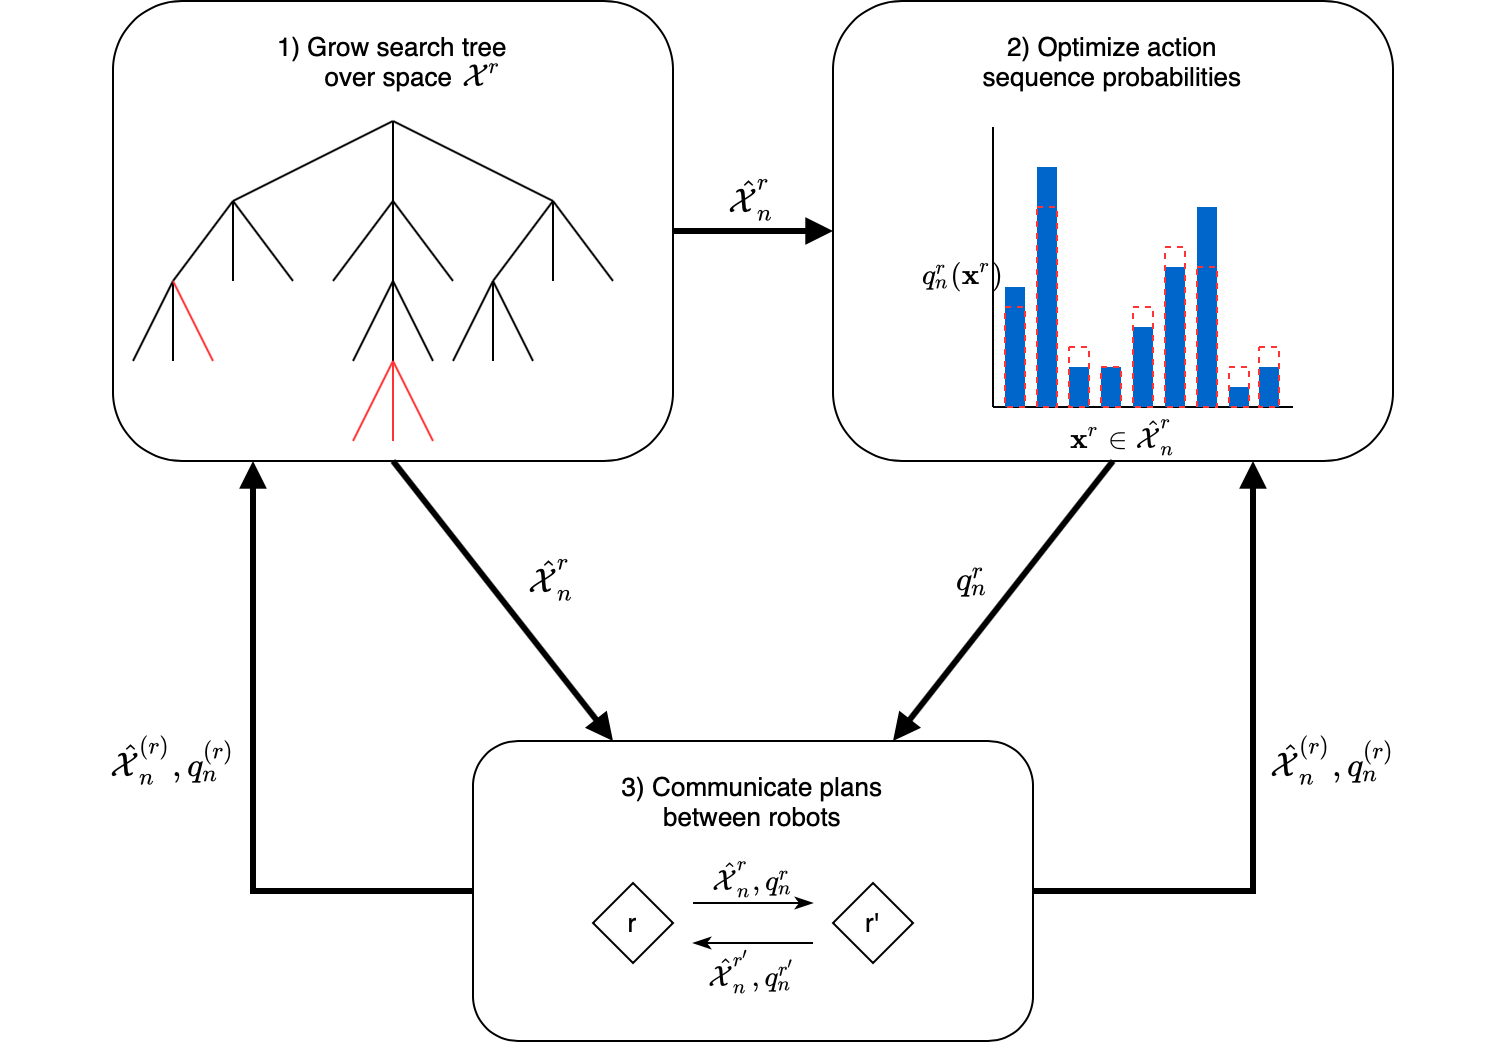
\includegraphics[width=0.9\textwidth]{img/dec-mcts.png}
    \caption{The three basic steps of Dec-MCTS.}
    \label{fig:dec_mcts}
\end{figure}
\subsection{Heuristics}
\label{ss:heuristics}
\paragraph{GRAVE}
RAVE and its generaliztion GRAVE \cite{cazenave2015generalized} are both answers to the following AMAF-tradeoff: Consider a node representing state $s$ at any point in the search tree. If we want to combine its UCT value and the AMAF-value of its predecessors it is not obvious which predecessor we should choose: If we choose the direct predecessor $s'$ (as does RAVE) its AMAF-value is similar to that of $s$ but less accurate overall since the number of times $s'$ was used in a simulation or chosen directly decreases the deeper we traverse the search tree. If we go further up the tree, i.e. choose more distant predecessors, the relationship between $s$ and $s'$ becomes more distant which usually means that the associated AMAF-values are also less close. However, $s'$ is part of simulations more often so all associated values are more precise in general. GRAVE addresses these problems by relying on an additional parameter \textit{ref}. It picks $s'$ as the closest predecessor that has been used at least \textit{ref} times in simulations. It is thus a true generalization as setting \textit{ref} to zero results in RAVE. In experiments with Go GRAVE performs better than either RAVE or UCT.
\paragraph{Parameter Randomization and GGP}
\cite{sironi2019comparing} focus on MCTS as a search strategy in \textit{General Game Playing} (GGP), that is the creation of agents that learn to play a variety of games while being given only their rules. These agents usually have only a limited time to prepare and execute their moves. To this end they need good (i.e. fast and accurate) search strategies to predict the course of the game. When MCTS is used in this scenario the actual actions taken by the search are controlled by the user via a number of parameters. Which values of these parameters are optimal depends on the game but since this is unknown in advance parameter tuning is often simply done offline by taking some aggregate of parameters tested on a set of games. An alternative approach is online tuning of parameters, i.e. adapting the MCTS-variant used while actually playing the game. However, since the time available for adjustments is so short randomizing parameters often results in similar performance. It should be noted however that this does not mean just assigning truly random numbers but rather the specific mapping of parameters to a set of possible values depending on the game and the role the agent plays in it. There are four general strategies for randomizing parameters:
\begin{itemize}
    \item \textit{Per run}: Update once before the game is started.
    \item \textit{Per turn}: Update every time the agent has to take a turn.
    \item \textit{Per simulation}: Update every time a new simulation is started (similar to online tuning).
    \item \textit{Per state}: Update every time a state is visited during a simulation.
\end{itemize}
Experimentally they show that tuning the parameters once \textit{per simulation} leads to the best performance.
\subsection{Planning}
\paragraph{Hierarchical Planning}
\cite{vien2015hierarchical} adapt MCTS to efficiently scale to large domains. Basic, that is flat, MCTS requires the explicit search for (many) reward states potentially located very far from the root node. This consumes a lot of computing resources To reduce the required effort we can exploit possible hierarchical structures of the domain called subtasks. The idea is to compute policies for whole subtasks purely based on sampling.

Traditionally, UCT has been effective at defeating both the \textit{curse of dimensionality} (where the complexity grows exponentially with the state space) and the \textit{curse of history} (where the complexity grows exponentially with the planning horizon). However, 
\todo{content, restructure, delete?}
\paragraph{MCTS-Alternative}
MCTS explores the most promising paths through game trees via policy-guided simulation (\textit{the default policy}). To adapt future searches certain pieces of data (i.e., monte carlo averages) need to be stored in the tree's nodes. In domains with a high branching factor this does not scale well. \cite{anthony2019policy} proposes a new search method called Policy Gradient Search (PGS). While this is also simulation-based the simulation is being done via a neural network and is adapted via online policy gradient updates. So no search tree is needed.
\todo{content, restructure?}
\subsection{MAB and UCB-Tuning}
\paragraph{Contexts} 
\cite{slivkins2014contextual}
In a multi-armed bandit (MAB) problem, an online algorithm makes a sequence of choices. In each round it chooses from a time-invariant set of alternatives and receives the payoff associated with this alternative. While the case of small strategy sets is by now well understood, a lot of recent work has focused on MAB problems with exponentially or infinitely large strategy sets, where one needs to assume extra structure in order to make the problem tractable. In particular, recent literature considered information on similarity between arms.
We consider similarity information in the setting of contextual bandits, a natural extension of the basic MAB problem where before each round an algorithm is given the context -a hint about the payoffs in this round. Contextual bandits are directly motivated by placing advertisements on web pages, one of the crucial problems in sponsored search. A particularly simple way to represent similarity information in the contextual bandit setting is via a similarity distance between the context-arm pairs which bounds from above the difference between the respective expected payoffs.
\todo{abstract, content}
\paragraph{Stochastics}
\cite{kaufmann2017monte} define a whole class of MCTS-algorithms called \textit{BAI-MCTS} (short for Best Arm Identification MCTS). For two player, zero-sum turn-based games the game tree $\mathcal{T}$ can be divided into MAX node where player A should take action and MIN nodes where player B should do so. ...
\todo{content}
\paragraph{Fixed Budgets}
The \textit{fixed budget} setting (as opposed to \textit{fixed confidence}) describes the constraint of a MAB-problem that the best possible arm must be identified using no more than $m$ \enquote{pulls}.
\cite{karnin2013almost} provides an almost optimal exploration algorithm in this setting called \textit{Sequential Halving} given in Algorithm \ref{alg:sequential_halving} . W.l.o.g the $k$ different arms are ordered according to their expected value $p_i$ at every decision epoch $t$: $p_1, \geq p_2 \geq \ldots \geq p_k$. $\Delta_i \coloneqq p_1 - p_i$ denotes the suboptimality gap of arm $i$. Consequently, $\Delta_2$ is the smallest of all these gaps. It can be shown that for the required budget $T$ for identifying the best arm with a probability of at least $(1-\delta)$ we have $T \in \Omega(H \log (\frac{1}{\delta}))$ where $H \coloneqq \sum_{i=2}^{k} \frac{1}{\Delta_i^2}$. $H$ is a measure of the complexity of the problem. Another related measure is given via: $H_2 \coloneqq \max_{i \neq 1} \frac{i}{\Delta_i^2}$. With these considerations we can now analyse the algorithm: Given a budget of $T$ pulls it identifies the best arm with a probability of at least $1-3 \log_2 k \cdot \exp \left(-\frac{T}{8H_2 \log_2 k}\right)$. 

\begin{algorithm}[htbp]
\begin{algorithmic}
\Function{SequentialHalving}{$T$} 
    \State $S_0 \gets [k]$
    \For{$r = 0$ to $\ceil*{\log_2 k} - 1$}
    \State $t_r = \floor*{\frac{T}{\left|S_r\right| \ceil*{log_2 k}}}$
    \State sample every arm $i \in S_r$ $t_r$ times
    \State calculate average reward $\Hat{p}_i^r$
    \State $S_{r+1} \gets \ceil*{\frac{\left| S_r \right|}{2}}$ arms in $S_r$ with largest average reward
    \EndFor
    \State \Return arm in $S_{\ceil*{\log_2 k}}$
\EndFunction
\end{algorithmic}
\caption{Sequential Halving.}
\label{alg:sequential_halving}
\end{algorithm}

\paragraph{Fixed Confidence}
\cite{jamieson2014lil} devises an optimal exploration algorithm called LIL'UCB for stochastic MAB-problems with a \textit{fixed confidence}. More precisely they define, a procedure with a single input $\delta > 0$ that solves the best arm problem with a confidence of $\delta$. That is, it identifies the arm with the largest mean with a probability of at least $1-\delta$ irrespective of the actual mean payoff of the arms $\mu_1,\ldots,\mu_K \in [0,1]$. A key concept here is the \textit{sampling} of arms, i.e. the realization of a Gaussian random variable with mean $\mu_i$ for arm $i$. Let $X_{i,s}$ denote independent samples from arm $i$ and let $T_i(t)$ denote the number of samples arm $i$ has been sampled up to time $t$. Then the empirical mean of these samples can be written as
\begin{equation*}
    \Hat{\mu}_{i,T_i(t)} \coloneqq \frac{1}{T_i(t)}\sum_{s=1}^{T_i(t)} X_{i,s}
\end{equation*}
Now the problem can be solved as follows: Initially, sample each arm once, giving us $T_i(t) = 1$ for every arm $i$ and $t = k$. Then, while it holds that $T_i(t) < 1 + \lambda \sum_{j\neq i} T_j(t)$ for all $i$, sample arm $I_t$ with
\begin{equation*}
    I_t = \underset{i \in \{1,\ldots,k\}}{\arg \max} \left\{ \Hat{\mu}_{i,T_i(t)} + (1+\beta)(1+\sqrt{\epsilon}) \sqrt{\frac{2\sigma^2 (1+\epsilon) \log \left(\frac{\log((1+\epsilon)T_i(t))}{\delta}\right)}{T_i(t)}}\right\}\text{.}
\end{equation*}
Set $T_i(t+1) = T_i(t) + 1$ if $I_t = i$, otherwise $T_i(t+1) = T_i(t)$. If the condition above no longer holds, stop and yield ${\arg \max}_{i \in \{ 1,\ldots,k\}} T_i(t)$ as output. Using the \textit{law of iterated logarithms} (LIL) they prove that this procedure cannot be improved by more than a constant factor.  
\todo{move to non-stationary?}
\paragraph{Combinatorial Exploration} \cite{chen2014combinatorial}
\paragraph{Non-Stationary} \cite{auer2002finite} prove a lower bound for policy performance for non-stationary MAB-problems. If at each decision epoch $t$ the rewards $X_t^k$ are distributed via a Bernoulli distribution with mean $\mu_t^k$ we have for any policy $\pi$:
\begin{equation*}
    \mathcal{R}^\pi(V_T,T) \geq CK^{\frac{1}{3}}V_T^{\frac{1}{3}}T^{\frac{2}{3}}
\end{equation*}
\cite{besbes2019optimal} provide a policy with this optimal bound called \textit{Rexp3}. Concretely, it defines a distribution over the $K$ arms $\{p_t^k\}_{k=1}^K$ with
\begin{equation*}
    p_t^k = (1-\gamma)\frac{w_t^k}{\sum_{k'=1}^K w^{k'}_t} +\frac{\gamma}{K}
\end{equation*} according to which the arms are drawn. Their weights are then updated as follows:
\begin{equation*}
    w_{t+1}^k = w_t^k \exp{\left\{\frac{\gamma \Hat{X}_t^k}{K}\right\}}
\end{equation*}
with $\Hat{X}_t^{k'} = \frac{X_t^{k'}}{p_t^{k'}}$. The value of the parameter $\gamma$ is given via $\gamma = \min \left\{1, \sqrt{\frac{K \log K}{(e-1)\Delta}} \right\}$. The additional parameter $\Delta$ in this definition refers to the batch-size. That is, $\gamma$ is updated every $\Delta = \ceil*{(K \log K)^\frac{1}{3} (\frac{T}{V_T})^\frac{2}{3}}$ epochs. Intuitively, $\gamma$ represents the exploration rate and $p_t^k$ represents the certainty of the policy that $k$ is optimal. 
\subsection{Evolutionary Algorithms}
\cite{lucas2014fast} describe a way of incorporating an evolutionary algorithms into  MCTS in place of a heuristic. Multiple variations (\enquote{individuals}) of the same MCTS-algorithm with different parameters are instantiated. Then their performance (their \enquote{fitness}) is evaluated using a metric and only the best ones get to \enquote{reproduce} and/or are modified using \enquote{mutations}. There are two general ways of evaluating fitness: Either the fitness of the algorithm is evaluated over a set of games and the actual effects of the algorithm (or MCTS-\textit{agent}) are viewed as a black box whose parameters can be tuned. Or, and this is the approach taken here, the evaluation happens during the simulation (i.e. step 3 in the description given above). Each individual is defined via a parameter-vector and is evaluated \begin{enumerate*}[label=\alph*)]
    \item on the same tree
    \item every time the default policy is executed 
\end{enumerate*}. Consequently, there is much more information available and the evolution can happen faster. The executed steps are displayed in Algorithm \ref{alg:fastevo_mcts}. At first a parameter vector $w$ is drawn and a new statistics-object $S$ is initialized. Now the tree and default policies controlled by $w$ are sampled $K$ times and the resulting metrics (such as min/max, average reward) are used to evaluate the fitness of the parameter vector. After the budget (time or computational resources) is used up the best vector is chosen and returned.
\begin{algorithm}[htbp]
\begin{algorithmic}
\Function{FastEvoMCTS}{$K, v_0$} 
    \While{within computational budget}
    \State $w \gets$ \Call{evo.getNext}{\null}
    \State Initialize $S$
    \For{$i \coloneqq 1$ to $K$}
    \State $v_l \gets$ \Call{TreePolicy}{$v_0,T(w)$}
    \State $\Delta \gets$ \Call{DefaultPolicy}{$s(v_l),D(w)$}
    \State \Call{Backup}{$S,\Delta$}
    \State \Call{UpdateStats}{$S,\Delta$}
    \EndFor
    \State \Call{evo.setFitness}{$\mathbf{w},S$}
    \EndWhile
    \State $\mathbf{w} \gets$ \Call{evo.getBest}{\null}
    \State $a \gets$ \Call{recommend}{$v_0$}
    \State \Return $(w,a)$
\EndFunction
\end{algorithmic}
\caption{Fast Evolutionary MCTS.}
\label{alg:fastevo_mcts}
\end{algorithm}

\cite{benbassat2014evomcts} presents another evolutionary approach to MCTS that focusses on zero-sum, deterministic, full-knowledge board games while remaining scalable.